\chapter{Planificación}

\subsection{Tareas}
\begin{table}[htbp]
	\begin{center}
		\begin{tabular}{| p{1.8cm}| p{1.2cm}| p{2.4cm}|p{2.2cm} |p{7.8cm} |}
			\hline
			\textbf{Requisito} & \textbf{Tarea} & \textbf {Responsable}& \textbf{Estimado} & \textbf{Descripcion}
			\\\hline  
			HU-4&T-1&Torres&7 horas&Lograr la traducción correcta de esta informacion en las lenguas Castellano y Quechua.
			\\ \hline
			HU-4&T-1&Vilca&5 horas&Buscar informacion acerca de la anemia y diabetes.
			\\ \hline
		\end{tabular}
	\end{center}
\end{table}
\begin{table}[htbp]
	\begin{center}
		\begin{tabular}{| p{1.8cm}| p{1.2cm}| p{2.4cm}|p{2.2cm} |p{7.8cm} |}
			\hline
			\textbf{Requisito} & \textbf{Tarea} & \textbf {Responsable}& \textbf{Estimado} & \textbf{Descripcion}
			\\\hline  
			HU-2 y 3&T-3&Flores&5 horas&Realizar una interfaz de login movil.
			\\ \hline
			HU-2 y 3&T-3&Vilca&5 horas&Desarrollo de la base de datos con las tablas.
			\\\hline  
			HU-2 y 3&T-3&Flores&4 horas&Realizar una interfaz de registro movil.
			\\ \hline
			HU-2 y 3&T-3&Torres&5 horas&Realizar una interfaz de login web.
			\\ \hline
			HU-2 y 3&T-3&Torres&5 horas&Realizar una interfaz de registro web.
			\\ \hline
		\end{tabular}
	\end{center}
\end{table}
\begin{table}[htbp]
	\begin{center}
		\begin{tabular}{| p{1.8cm}| p{1.2cm}| p{2.4cm}|p{2.2cm} |p{7.8cm} |}
			\hline
			\textbf{Requisito} & \textbf{Tarea} & \textbf {Responsable}& \textbf{Estimado} & \textbf{Descripcion}
			\\\hline  
			HU-5&T-5&Torres&6 horas&Realización de la interfaz para los cuestionarios para las enfermedades web.
			\\ \hline
			HU-7&T-7&Torres&10 horas&Realizar la interfaz de los cuadros estadísticos sobre los resultados generales de todos los usuarios participantes y también de manera personal para cada usuario.
			\\ \hline
		\end{tabular}
	\end{center}
\end{table}
\begin{figure}
	\centering
	\includegraphics[width=1.1\linewidth]{C:/Users/USUARIO/Documents/Trello}
	\caption[Figura 1]{Trello del proyecto Primer Spring}
	\label{fig:trello}
\end{figure}

\begin{figure}
	\centering
	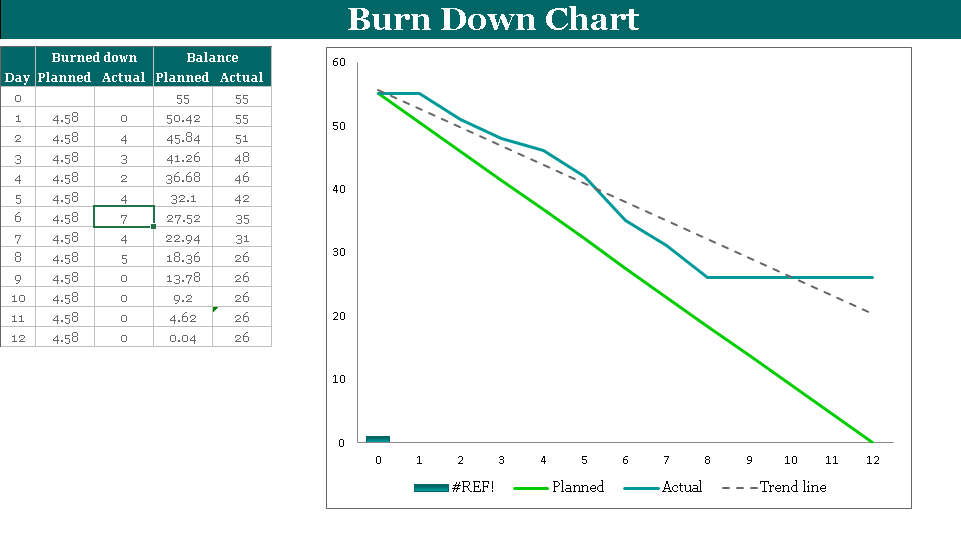
\includegraphics[width=1.2\linewidth]{img/Burndown}
	\caption[Figura 2]{Burndown}
	\label{fig:burndown}
\end{figure}

\begin{figure}
	\centering
	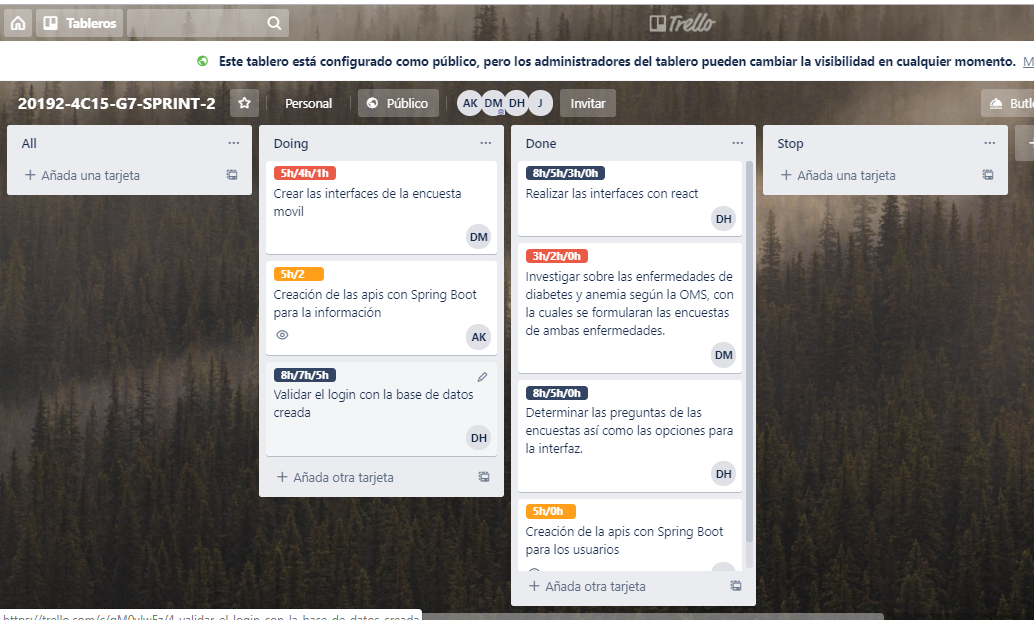
\includegraphics[width=1.1\linewidth]{img/Spring2}
	\caption[Figura 3]{Trello del proyecto Segundo Spring}
	\label{fig:spring2}
\end{figure}




